\section{Images and tables}

\subsection{Approximations for the TBCs - Constant and linear polynomial}

\begin{minipage}{.5\linewidth}
	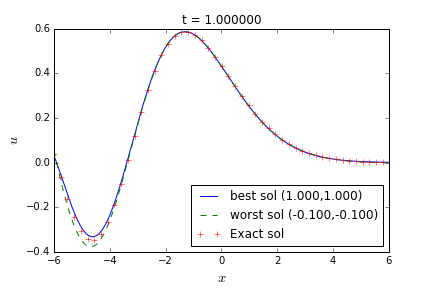
\includegraphics[scale=.5]{figures/firstTestsP0Snap2.png}
\end{minipage}
\begin{minipage}{.5\linewidth}
	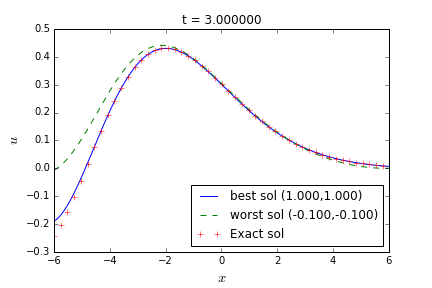
\includegraphics[scale=.5]{figures/firstTestsP0Snap4.png}
\end{minipage}
\captionof{figure}{Best and worst solution compared with analytical solution, for the constant polynomial approximation}

%\begin{minipage}{.5\linewidth}
%	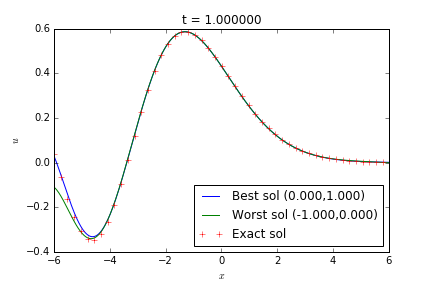
\includegraphics[scale=.5]{figures/firstTestsP1Snap0.png}
%\end{minipage}
%\begin{minipage}{.5\linewidth}
%	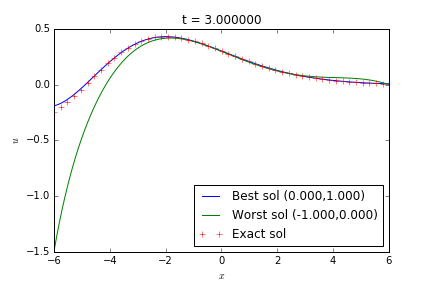
\includegraphics[scale=.5]{figures/firstTestsP1Snap2.png}
%\end{minipage}
%\captionof{figure}{Best and worst solution compared with analytical solution, for the linear polynomial approximation}

\sisetup{round-mode=places}
\begin{center}
\begin{tabular}{c|c|S[round-precision=4,table-number-alignment =  left]}
	\multicolumn{1}{c|}{$c_L$}  & \multicolumn{1}{c|}{$c_R$} & \multicolumn{1}{r}{$e_{L2}$} \\
	\hline
	1.0 & 1.0 & 0.0946839239675 \\
	1.0 & 10.0 & 0.097288371204 \\
	1.0 & 0.1 & 0.0983932287563 \\
	1.0 & 0.0 & 0.0992063806502 \\
	1.0 & -10.0 & 0.099359192771 \\
	1.0 & -0.1 & 0.100021589665 \\
	1.0 &  -1. & 0.10159265619 \\
	10.0 & 1.0 & 0.347003021321 \\
	10.0 & 0.1 & 0.347379492262 \\
	10.0 & 0.0 & 0.347487945035
\end{tabular}
\captionof{table}{Best results (smallest $e_{L2}$) for the constant polynomial approximation \label{tab:firstTestsP0}}
\end{center}

	 \sisetup{round-mode=places}
\begin{center}
\begin{tabular}{c|c|S[round-precision=4,table-number-alignment =  left]}
	\multicolumn{1}{c|}{$d_L = d_R$}  & \multicolumn{1}{c|}{$c_L = c_R$} & \multicolumn{1}{r}{$e_{L2}$} \\
	\hline
	0. & 1.0 & 0.0946839239675 \\
	0.1 & 1.0 & 0.12341195 \\
	1.0 & 1.0 & 0.20031603 \\
	10.0 & 0.1 & 0.22037249 \\
	-10.0 & 0.1 & 0.23984486 \\
	10.0 & 1.0 & 0.27161158 \\
	-10.0 &  0.0 & 0.24800816\\
	-10.0 & 1.0 & 0.30039637 \\
	10.0 & 0.0 & 0.27213611 \\
	0.0 & 0.1 & 0.36740764
\end{tabular}
\captionof{table}{Best results (smallest $e_{L2}$) for the linear polynomial approximation \label{tab:firstTestsP1}}
\end{center}


\newpage

\subsection{Optimization of the coefficients for the TBC (minimization of the error compared to the analytical solution)}

\begin{minipage}{.5\linewidth}
	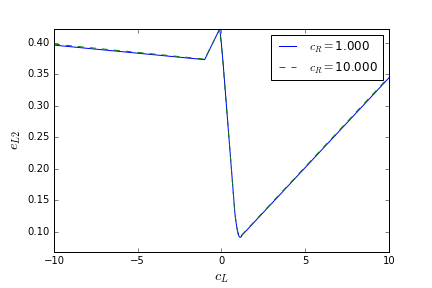
\includegraphics[scale=.45]{figures/errorOptimOnlyL2.png}
	\captionof{subfigure}{General view of all the tested coefficients}
\end{minipage}
\begin{minipage}{.5\linewidth}
	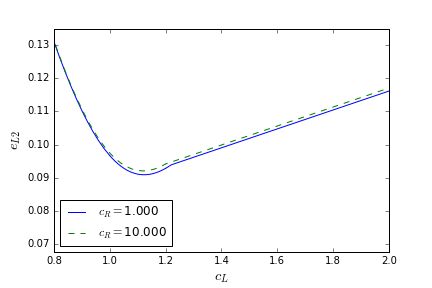
\includegraphics[scale=.45]{figures/errorOptimOnlyL2Detail.png}
	\captionof{subfigure}{Detail for $c_L \in [0.8,2.0]$}
\end{minipage}
	\captionof{figure}{Error of the numerical solution compared to the analytical solution as function of the constant polynomial approximation for the TBC}



\newpage

\subsection{Numerical verification of the error in the DDM}

%\begin{center}
%	\begin{tabular}{c|S[round-precision=4]|S[round-precision=4]}
%	\multicolumn{1}{c|}{}  & \multicolumn{1}{c|}{$\Omega_1\bigcap \Omega_2$} & \multicolumn{1}{c}{$\Omega$} \\
%	\hline
%	$e^{125}/e^{250}$ & 2.85579232 & 2.58072011\\
%	$e^{250}/e^{500}$ & 2.30413455 & 2.22892 \\
%	$e^{500}/e^{1000}$ &  2.13697696 & 2.11557312 \\
%	$e^{1000}/e^{2000}$ & 2.06417829 & 2.05805538\\
%	$e^{2000}/e^{4000}$ & 2.03095261 & 2.02909704 \\
%	$e^{4000}/e^{8000}$ & 2.01518696 & 2.01456961 \\
%	\end{tabular}
%	\captionof{table}{Numerical verification of the order of convergence of the error due to the Domain Decomposition Method\label{tab:orderVerification}}
%\end{center}

\begin{center}
	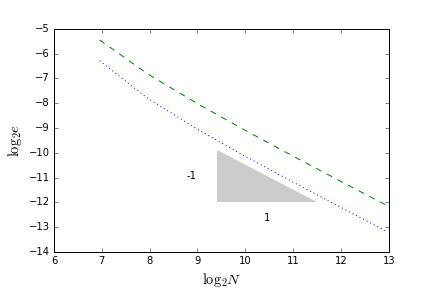
\includegraphics[scale=.5]{figures/convergenceVerification.png}
	\captionof{figure}{Numerical verification of the order of convergence of the error due to the Domain Decomposition Method}
\end{center}


\subsection{Optimization of the TBCs for the DDM (speed of convergence)}

\begin{minipage}{.5\linewidth}
\begin{center}
	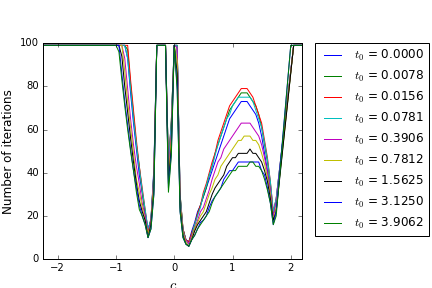
\includegraphics[scale=.4]{figures/NiterxCoefVarT0NegativeCoef.png}
	\captionof{subfigure}{General view for positive and negative coefficients }
\end{center}
\end{minipage}
\begin{minipage}{.5\linewidth}
\begin{center}
	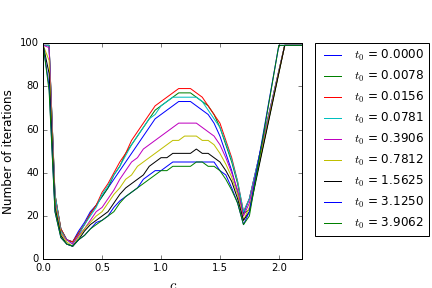
\includegraphics[scale=.4]{figures/NiterxCoefVarT0.png}
	\captionof{subfigure}{Detail for $c \geq 0.$ }
\end{center}
\end{minipage}
\captionof{figure}{Number of iterations until the convergence as function of the coefficient of the TBC (for a fixed interface and different values of $t_0$) }

\begin{minipage}{.5\linewidth}
\begin{center}
	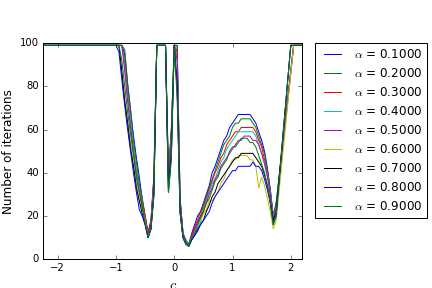
\includegraphics[scale=.4]{figures/NiterxCoefVarInterfaceNegativeCoef.png}
	\captionof{subfigure}{General view for positive and negative coefficients }
\end{center}
\end{minipage}
\begin{minipage}{.5\linewidth}
\begin{center}
	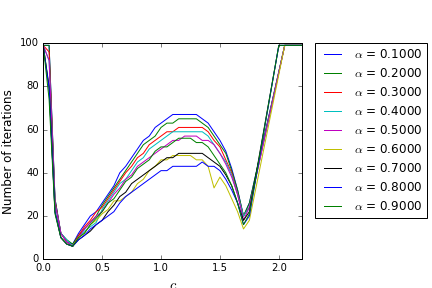
\includegraphics[scale=.4]{figures/NiterxCoefVarInterface.png}
	\captionof{subfigure}{Detail for $c \geq 0$ }
\end{center}
\end{minipage}
	\captionof{figure}{Number of iterations until the convergence as function of the coefficient of the TBC (for a fixed $t_0$ and different positions of the interface }

\begin{center}
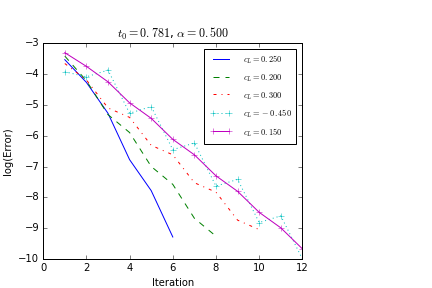
\includegraphics[scale=.5]{figures/errorEvolutionFixedT0BNegativeCoef.png}
\captionof{figure}{Error evolution with the iterations for the fastest results}
\end{center}

\begin{center}
	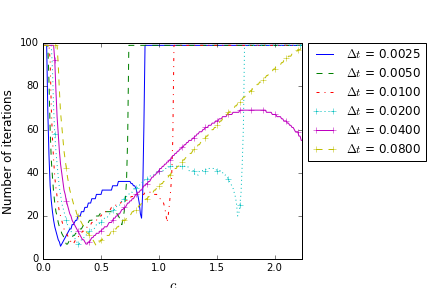
\includegraphics[scale=.5]{figures/NiterxCoefVarDtdx500.png}
\captionof{figure}{Number of iterations until the convergence as function of the coefficient of the TBC (for a fixed $N = 499$ and different values of $\Delta t$)}
\end{center}

\begin{center}
	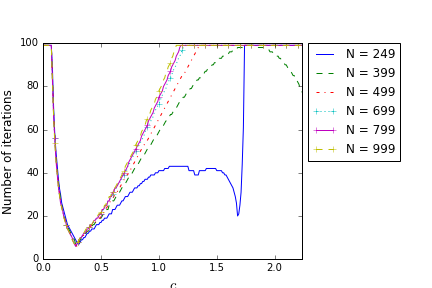
\includegraphics[scale=.5]{figures/NiterxCoefVarDxdt2em2.png}
\captionof{figure}{Number of iterations until the convergence as function of the coefficient of the TBC (for a fixed $\Delta t = 0.02$ and different values of $\Delta x$)}
\end{center}

\begin{center}
	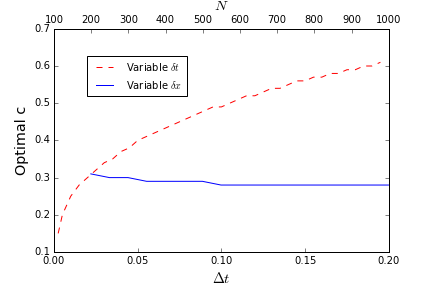
\includegraphics[scale=.5]{figures/OptimalCoefVarDxDt.png}
	\captionof{figure}{Optimal coefficients as function of the time step and the space step}
\end{center}